\documentclass{article}
\usepackage[latin1]{inputenc}
\usepackage[spanish,es-tabla]{babel}
\usepackage{amsmath}
\usepackage{amsfonts}
\usepackage{amssymb}
\usepackage{graphicx}
\usepackage{float}
\usepackage{hyperref}
\usepackage{subfig}
\usepackage[left=4cm,right=3cm,top=4cm,bottom=3cm]{geometry}
\author{Gatica, Isaias \\ Martin, Santiago \\ Saez, Lautaro Ándres \\ Vidman, Xavier Harry}
\title{Procesamiento digital de señales: estimación del espectro de una señal}
\date{}
\begin{document}
\maketitle
%\tableofcontents
El objetivo de este informe es analizar el uso de la DFT para estimar el espectro de una señal. Para ello se verán los cuatro casos posibles, según la señal sea continua o discreta, y periódica o aperiódica.


Se analizará en los distintos casos si es posible obtener una estimación sin error y bajo qué condiciones; qué efectos tienen parámetros como la frecuencia de muestreo y la cantidad de muestras; qué efecto tiene el método de zero-padding; y cómo utilizar correctamente la función \textit{fftshift}.


Además, cada ejercicio concluirá con el armado de una rutina que implemente la estimación del espectro usando la DFT.


\section{Ejercicio 1}
En este ejercicio se analiza el caso en que una señal es periódica y discreta. Se considera en primera instancia la siguiente señal: 

\begin{equation}
x[n]=sen(2 \pi n /8)
\label{eq.x[n]}
\end{equation}

\subsection*{Inciso a)}
En este inciso se calcula la DTFS y la DFT de la ecuación (\ref{eq.x[n]}). Se sabe con anterioridad que la DTFS de una señal está definida por las siguientes dos ecuaciones:

\begin{equation}
x[n] = \sum_{k=<N>}^{} c_{k} e^{jk \frac{2 \pi}{N} n}
\end{equation}

\begin{equation}
c_{k} = \frac{1}{N} \sum_{k=<N>}^{} x[n] e^{-jk \frac{2 \pi}{N} n}
\end{equation}	

Por lo tanto, para calcular la DTFS se deben calcular los coeficientes $c_{k}$. Como la señal de la ecuación (\ref{eq.x[n]}) es una señal senoidal, se puede expresar de la siguiente manera:

\begin{equation}
x[n]= \frac{1}{2j} \left( e^{(j \pi n)/4)}-e^{-(j \pi n)/4} \right)
\end{equation}

Por lo tanto, la DTFS de la señal de la ecuación (\ref{eq.x[n]}) es simplemente la ecuación (4); donde sus coeficientes $c_{k}$ son:

\begin{eqnarray}
C_{1}=\frac{1}{2j} \qquad C_{-1}=\frac{-1}{2j} \nonumber
\end{eqnarray}

La definición de la DFT que se utiliza es la siguiente:

\begin{equation}
X[k] = \sum_{n=0}^{N-1} x[n] e^{-jk \frac{2 \pi}{N} n}
\label{eq.DFT}
\end{equation}

donde N no representa necesariamente el período de la señal, si no que representa la cantidad de muestras consecutivas tomadas de la señal $x[n]$.


Para calcular la DFT, en primera instancia se aplica la ecuación (\ref{eq.DFT}), donde se obtiene: 

\begin{equation}
    x[k] = \sum_{n=0}^{7} \sin \left( \frac{\pi }{4} n \right) e^{-j\frac{\pi }{4}nk} 
\end{equation}

Para desarrollar la sumatoria de forma más sencilla la sumatoria presentan los valores de $x[n]$ para $n \in \{0, 1, 2, 3, 4 , 5, 6, 7\}$ en la 
Tabla (\ref{tab.xn}).

\begin{table}[H]
    \centering
    \begin{tabular}{|c|c|c|c|c|c|c|c|c|}
    \hline
    $n$    & 0 & 1                             & 2 & 3                             & 4 & 5                              & 6 & 7                              \\ \hline
    $x[n]$ & 0 & $\sqrt{2}/2$ & 1 & $\sqrt{2}/2$ & 0 & $-\sqrt{2}/2$ & 1 & $-\sqrt{2}/2$ \\ \hline
    \end{tabular}
    \caption{Valores de $x[n]$ para un periodo.}
    \label{tab.xn}
    \end{table}

Con lo que se obtiene 

\begin{equation}
    X[k]= \frac{\sqrt{2}}{2} e^{-j\frac{\pi }{4}k} + e^{-j\frac{\pi }{2}k} + \frac{\sqrt{2}}{2} e^{-j\frac{3\pi }{4}k}
    - \frac{\sqrt{2}}{2} e^{-j\frac{5\pi }{4}k} - e^{-j\frac{3\pi }{2}k} - \frac{\sqrt{2}}{2} e^{-j\frac{7\pi }{4}k} 
\end{equation}

Si expresamos las exponenciales correspondientes para $n \in \{ 5, 6 ,7 \}$ como $m\pi/4 + \pi$ donde $m$ es un entero entre 
$0$ y $4$, es posible expresar 

\begin{equation}
    X[k] = \frac{\sqrt{2}}{2} e^{-j\frac{\pi }{4}k} + e^{-j\frac{\pi }{2}k} + \frac{\sqrt{2}}{2} e^{-j\frac{3\pi }{4}k}
    - \frac{\sqrt{2}}{2} e^{-j\frac{\pi }{4}k} e^{-j\pi k} - e^{-j\frac{\pi }{2}k}e^{-j\pi k} - \frac{\sqrt{2}}{2} e^{-j\frac{3\pi }{4}k} e^{-j\pi k}
\end{equation}

Como $k$ es entero y $e^{-j\pi k}$ es siempre múltiplo de $\pi$ entonces $e^{-j\pi k} = (-1)^k$.

\begin{equation}
    X[k] = \frac{\sqrt{2}}{2} e^{-j\frac{\pi }{4}k} + e^{-j\frac{\pi }{2}k} + \frac{\sqrt{2}}{2} e^{-j\frac{3\pi }{4}k}
    (-1)^{1+k} \frac{\sqrt{2}}{2} e^{-j\frac{\pi }{4}k} +(-1)^{1+k} e^{-j\frac{\pi }{2}k} + (-1)^{1+k}\frac{\sqrt{2}}{2} e^{-j\frac{3\pi }{4}k} 
\end{equation}

Agrupando los valores se obtiene:

\begin{equation}
    X[k]= [ 1 + (-1)^{1+k} ] ( \frac{\sqrt{2}}{2} e^{-j\frac{\pi }{4}k} +e^{-j\frac{\pi }{2}k} + 
    \frac{\sqrt{2}}{2}  e^{-j\frac{3\pi }{4}k} )
    \label{eq.xk}
\end{equation}


Sabiendo que $X[k]$ es periódica con periodo $N$, en este caso $8$, se muestran en la Tabla (\ref{tab.xk}) los valores obtenidos para 
los diferentes valores de $k$ en un periodo, por otro lado de la ecuación (\ref{eq.xk}) se sabe que si $k$ es par $X[k]$ es $0$.

\begin{table}[]
    \centering
    \begin{tabular}{|c|c|c|c|c|c|c|c|c|}
    \hline
    $k$    & 0 & 1                             & 2 & 3                             & 4 & 5                              & 6 & 7                              \\ \hline
    $X[k]$ & 0 & $-4j$ & 1 & 0 & 0 & 0 & 0 & $4j$ \\ \hline
    \end{tabular}
    \caption{$X[k]$ obtenidos para un periodo.}
    \label{tab.xk}

\end{table}

%TERMINA LO DEL LAUTI

Al finalizar con el cálculo de la DFT, se pueden sustraer varias conclusiones entre la DFT y la DTFS. En primera instancia, al comparar la expresión de los $c_{k}$ de la DTFS con la expresión de la DFT, se puede ver una gran semejanza por el parecido entre las sumatorias de ambas. Pero hay dos grandes diferencias entre ellas. En primer lugar, los $c_{k}$ están multiplicados por el factor $\frac{1}{N}$, por lo que las amplitudes no serán coincidentes. En segundo lugar, para calcular los $c_{k}$ se debe usar obligatoriamente a N como el valor del período de la señal, y en la DFT no necesariamente; ya que el valor de N en la expresión de la DFT representa la cantidad de muestras consecutivas tomadas de la señal $x[n]$.

Al realizar los cálculos y comparar, se puede observar que si en la expresión de la DFT se utiliza el valor del período en N, los valores $c_{k}$ y los valores de $X(k)$ coinciden en el eje k, pero difieren en el valor de amplitud por el factor $\frac{1}{N}$ de la expresión (3).

\subsection*{Inciso b)}
En este inciso se genera la señal $x[n]=sen(2 \pi n /8)$ para $n$ de 0 a 7, y se calcula la DFT usando la función \textit{fft}.
En la Figura \ref{fig.1b} se visualiza la señal $x[n]$ para $n$ de 0 a 7.

\begin{figure}[H]
\centering
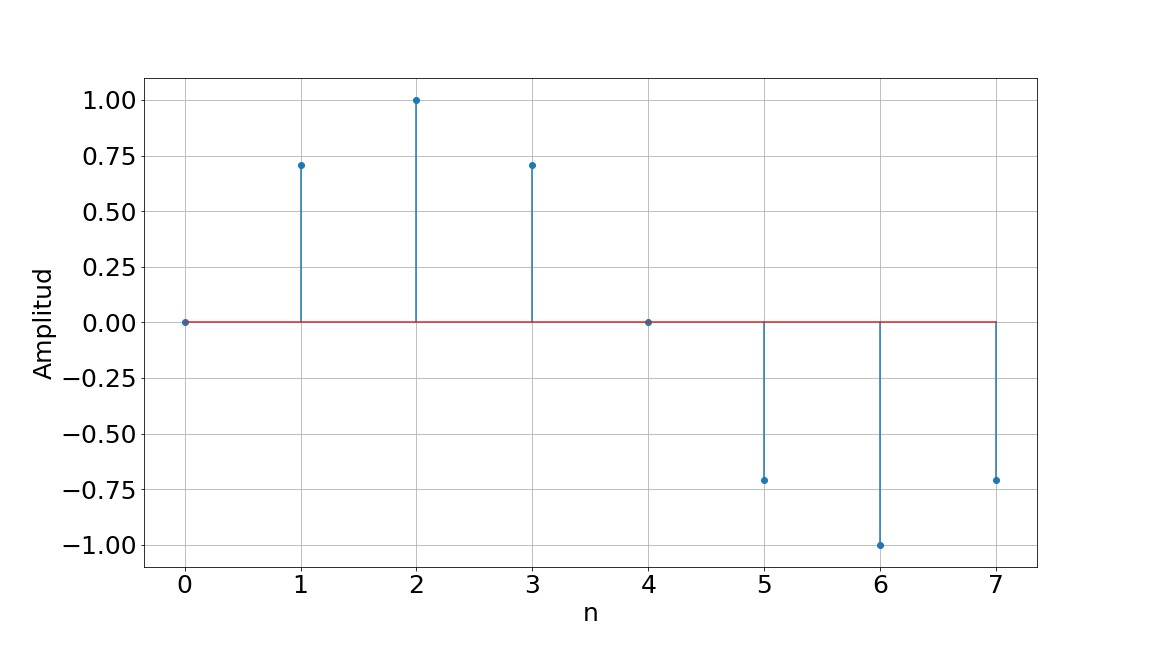
\includegraphics[width=0.75\textwidth]{Img/punto_1_b_signal.png}
\caption{Señal $x[n]$ generada para n de 0 a 7}
\label{fig.1b}
\end{figure}

El resultado del cálculo de la DFT utilizando la \textit{fft}, se puede observar en la Figura \ref{fig.2b}.

\begin{figure}[H]
\centering
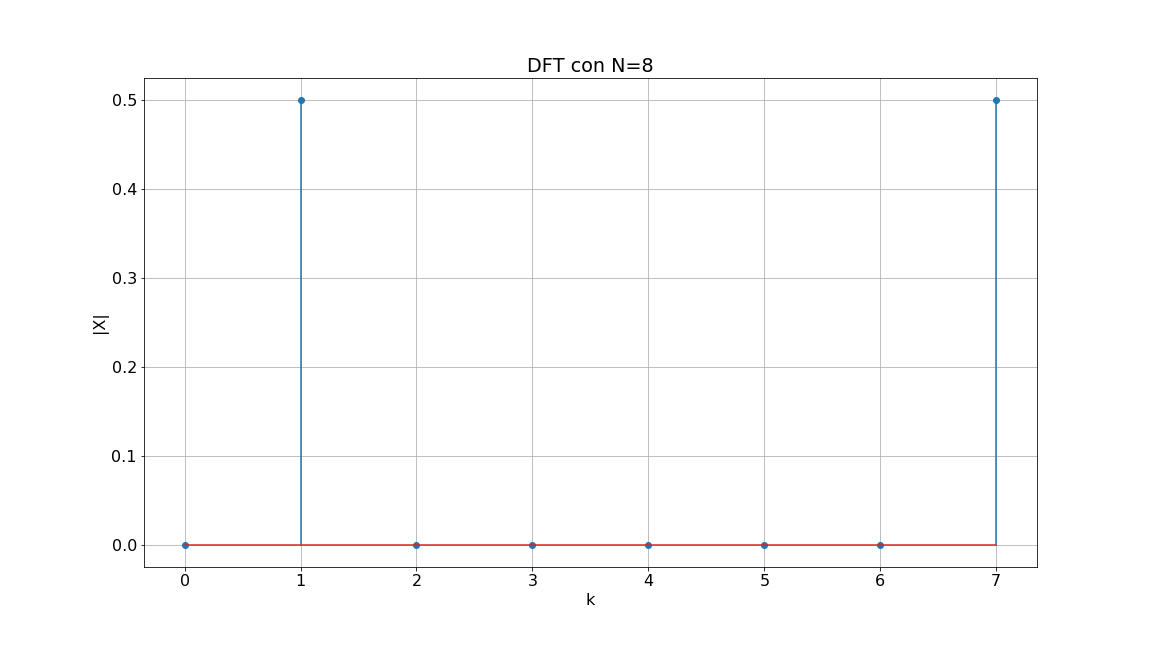
\includegraphics[width=0.75\textwidth]{Img/punto_1_b.png}
\caption{DFT de la señal $x[n]$ utilizando la \textit{fft} con N=8}
\label{fig.2b}
\end{figure}

Comparando la Figura \ref{fig.2b} con los resultados teóricos obtenidos en el inciso \textbf{a}, se puede afirmar que efectivamente se está calculando el espectro de la señal $x[n]$ al usar la \textit{fft} con N=8. Esto se debe a que la función \textit{fft} genera una señal periódica utilizando las muestras de la señal $x[n]$ que se le dieron como parámetro. 

%Mientras esas muestras sean un período o un múltiplo de un período, la señal periódica generada por la \textit{fft} coincidirá con la señal periódica original.

\subsection*{Inciso c)}
En este inciso se realiza lo mismo que en el inciso \textbf{b} pero esta vez, el valor de n es de 0 a 8. 


El resultado del cálculo de la DFT utilizando la \textit{fft}, con n de 0 a 8, se puede visualizar en la Figura \ref{fig.1c}.

\begin{figure}[H]
\centering
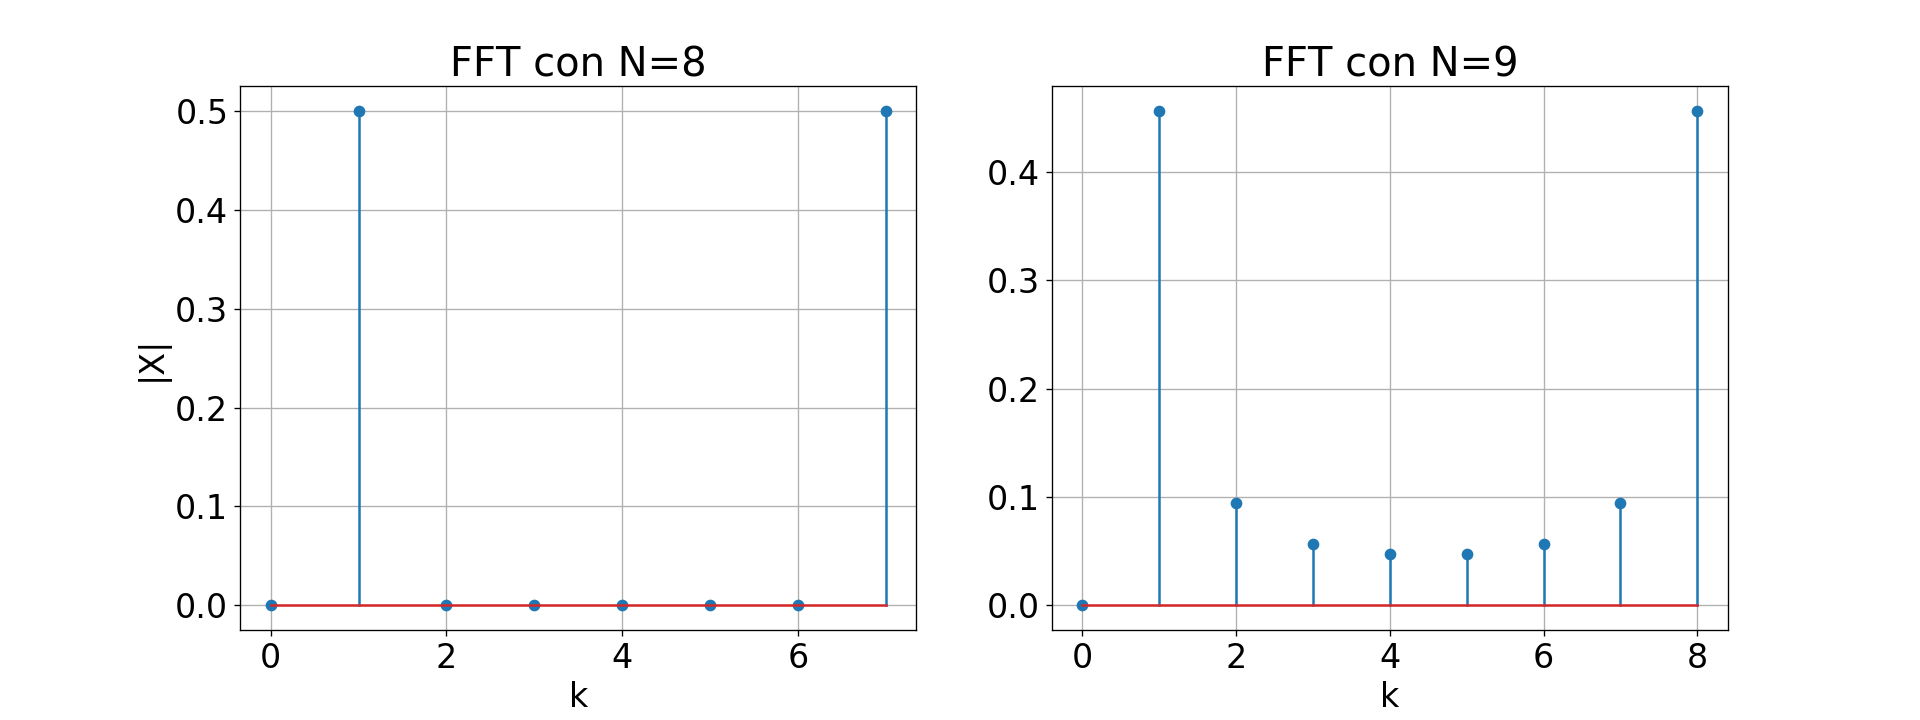
\includegraphics[width=0.75\textwidth]{Img/punto_1_c.png}
\caption{DFT de la señal $x[n]$ utilizando la \textit{fft} con N=9}
\label{fig.1c}
\end{figure}

Se puede observar que el gráfico obtenido difiere con el espectro de la señal original $x[n]$. Esto es consecuencia de haber modificado la cantidad de muestras consecutivas que se le da a la función \textit{fft}.

\subsection*{Inciso d)}
En esta sección se genera nuevamente la señal $x[n]$ con n de 0 a N, para los siguientes valores de N: 16, 24 y 160.


En la Figura \ref{fig.1d} se encuentran los resultados del cálculo de la DFT utilizando la \textit{fft} para los valores de N mencionados anteriormente. 

\begin{figure}[H]
\centering
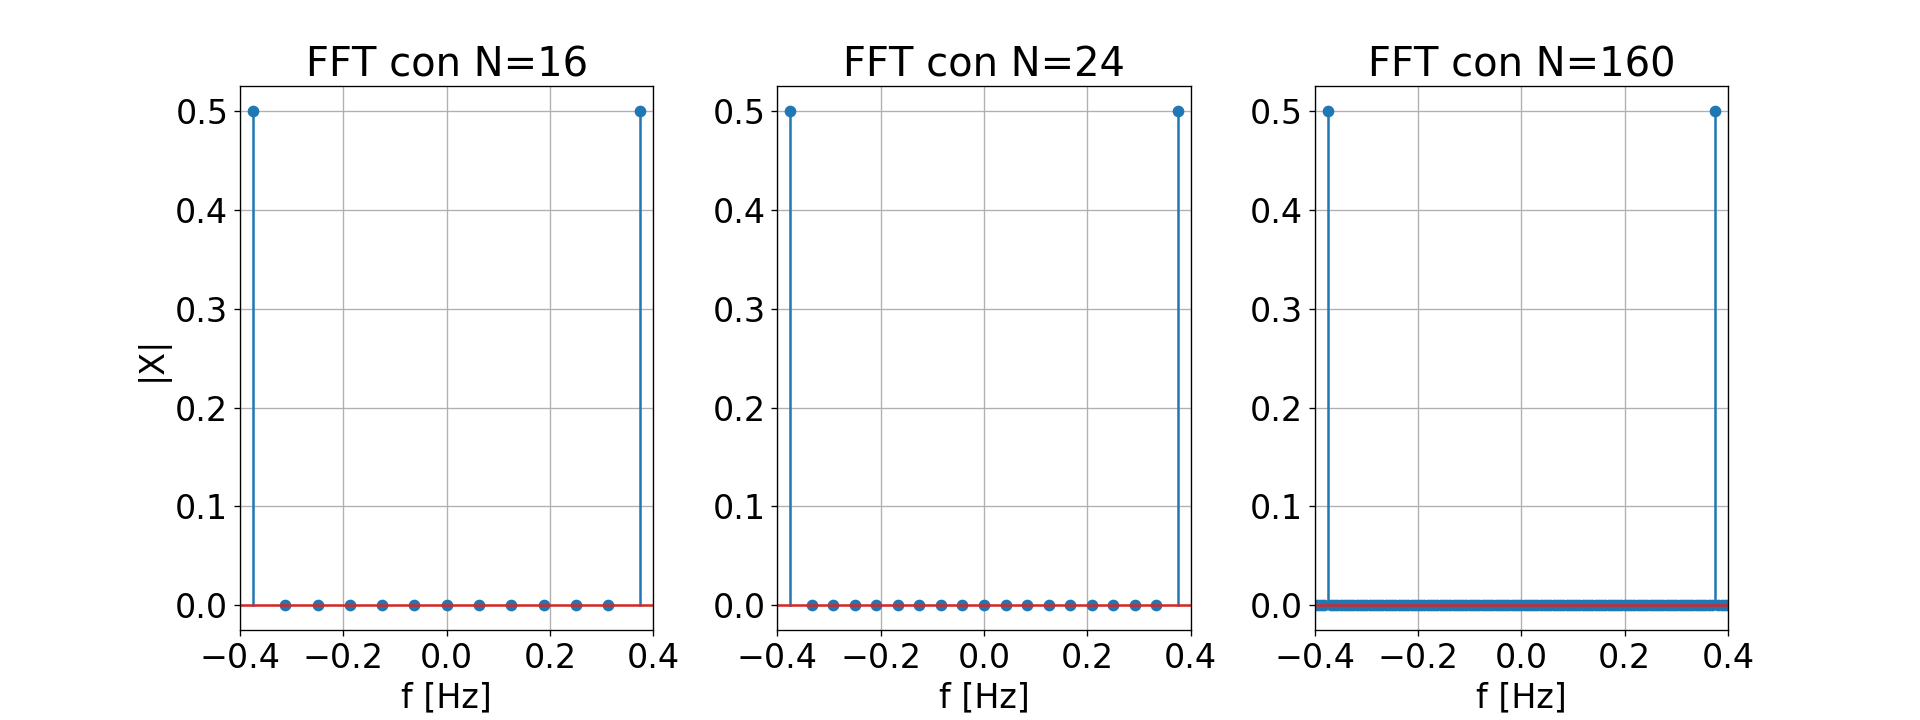
\includegraphics[width=0.75\textwidth]{Img/punto_1_d.png}
\caption{DFT de la señal $x[n]$ utilizando la \textit{fft} con los siguientes valores de N: 16, 24 y 160.}
\label{fig.1d}
\end{figure}

Se puede observar que los gráficos coinciden con lo analizado de forma teórica, y las tres simulaciones representan el espectro de la señal $x[n]$. La señal periódica generada por la \textit{fft} en los tres casos coincide con la señal periódica original, ya que la cantidad muestras que se ingresan a la función \textit{fft} son múltiplos del período fundamental de $x[n]$.

\subsection*{Inciso e)}
Cerrando con el análisis de la ecuación (\ref{eq.x[n]}), en este inciso se analiza qué sucede cuando se genera la señal $x[n]$ con n de 0 a N, para los siguientes valores de N: 17, 25 y 161.


En la Figura \ref{fig.1e} se encuentran los resultados del cálculo de la DFT utilizando la \textit{fft} para los valores de N mencionados anteriormente.

\begin{figure}[H]
\centering
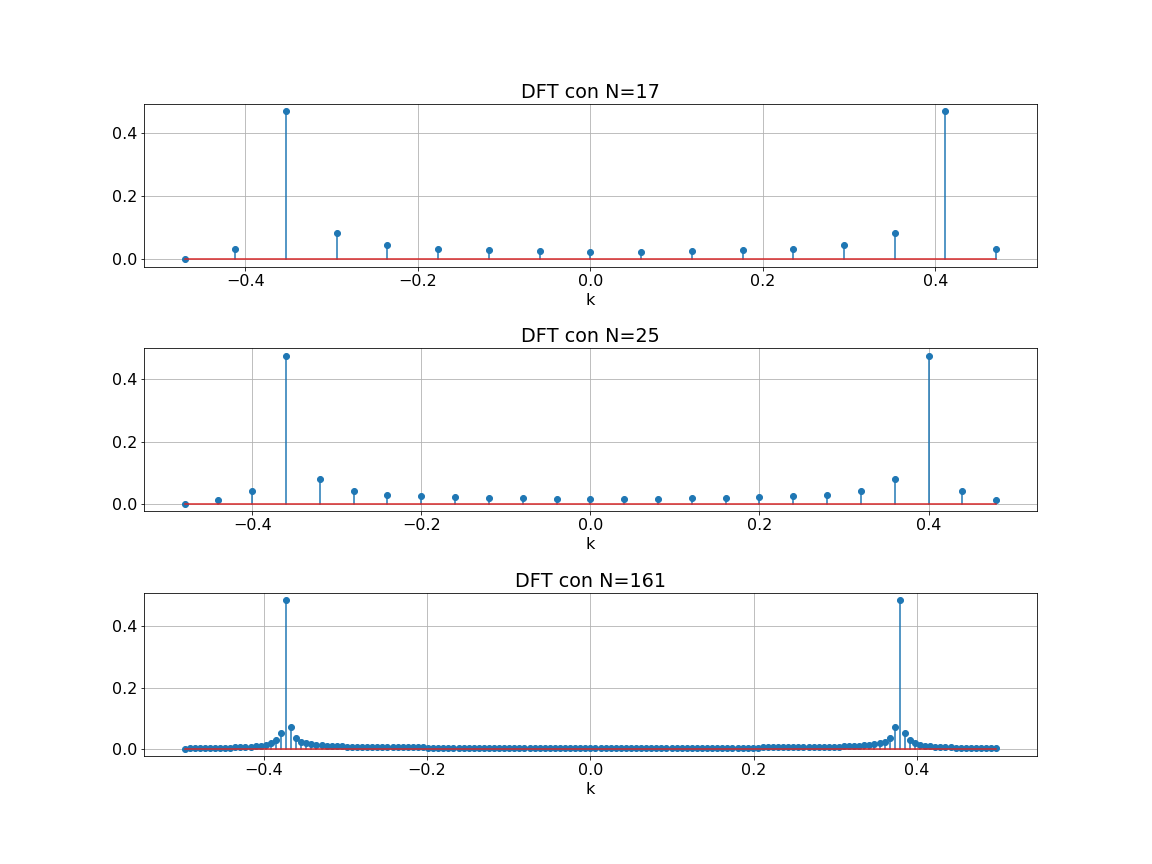
\includegraphics[width=0.75\textwidth]{Img/punto_1_e.png}
\caption{DFT de la señal $x[n]$ utilizando la \textit{fft} con los siguientes valores de N: 17, 25 y 161.}
\label{fig.1e}
\end{figure}

Si se comparan los gráficos mostrados en la Figura \ref{fig.1e} con el espectro de la señal $x[n]$ calculado teóricamente, se puede concluir que no se está obteniendo lo mismo. La \textit{fft} está mostrando en sus resultados componentes armónicos erróneos, consecuencia de la equívoca elección del valor de N utilizado para generar la señal periódica y cálculo de la DFT. La cantidad de muestras otorgadas como información al algoritmo, no representan un período de la señal. Por lo tanto, el algoritmo genera una señal periódica con un período distinto al original, y en consecuencia, un señal diferente.  Este fenómeno se observa en la Figura \ref{fig.2e}.

\begin{figure}[H]
\centering
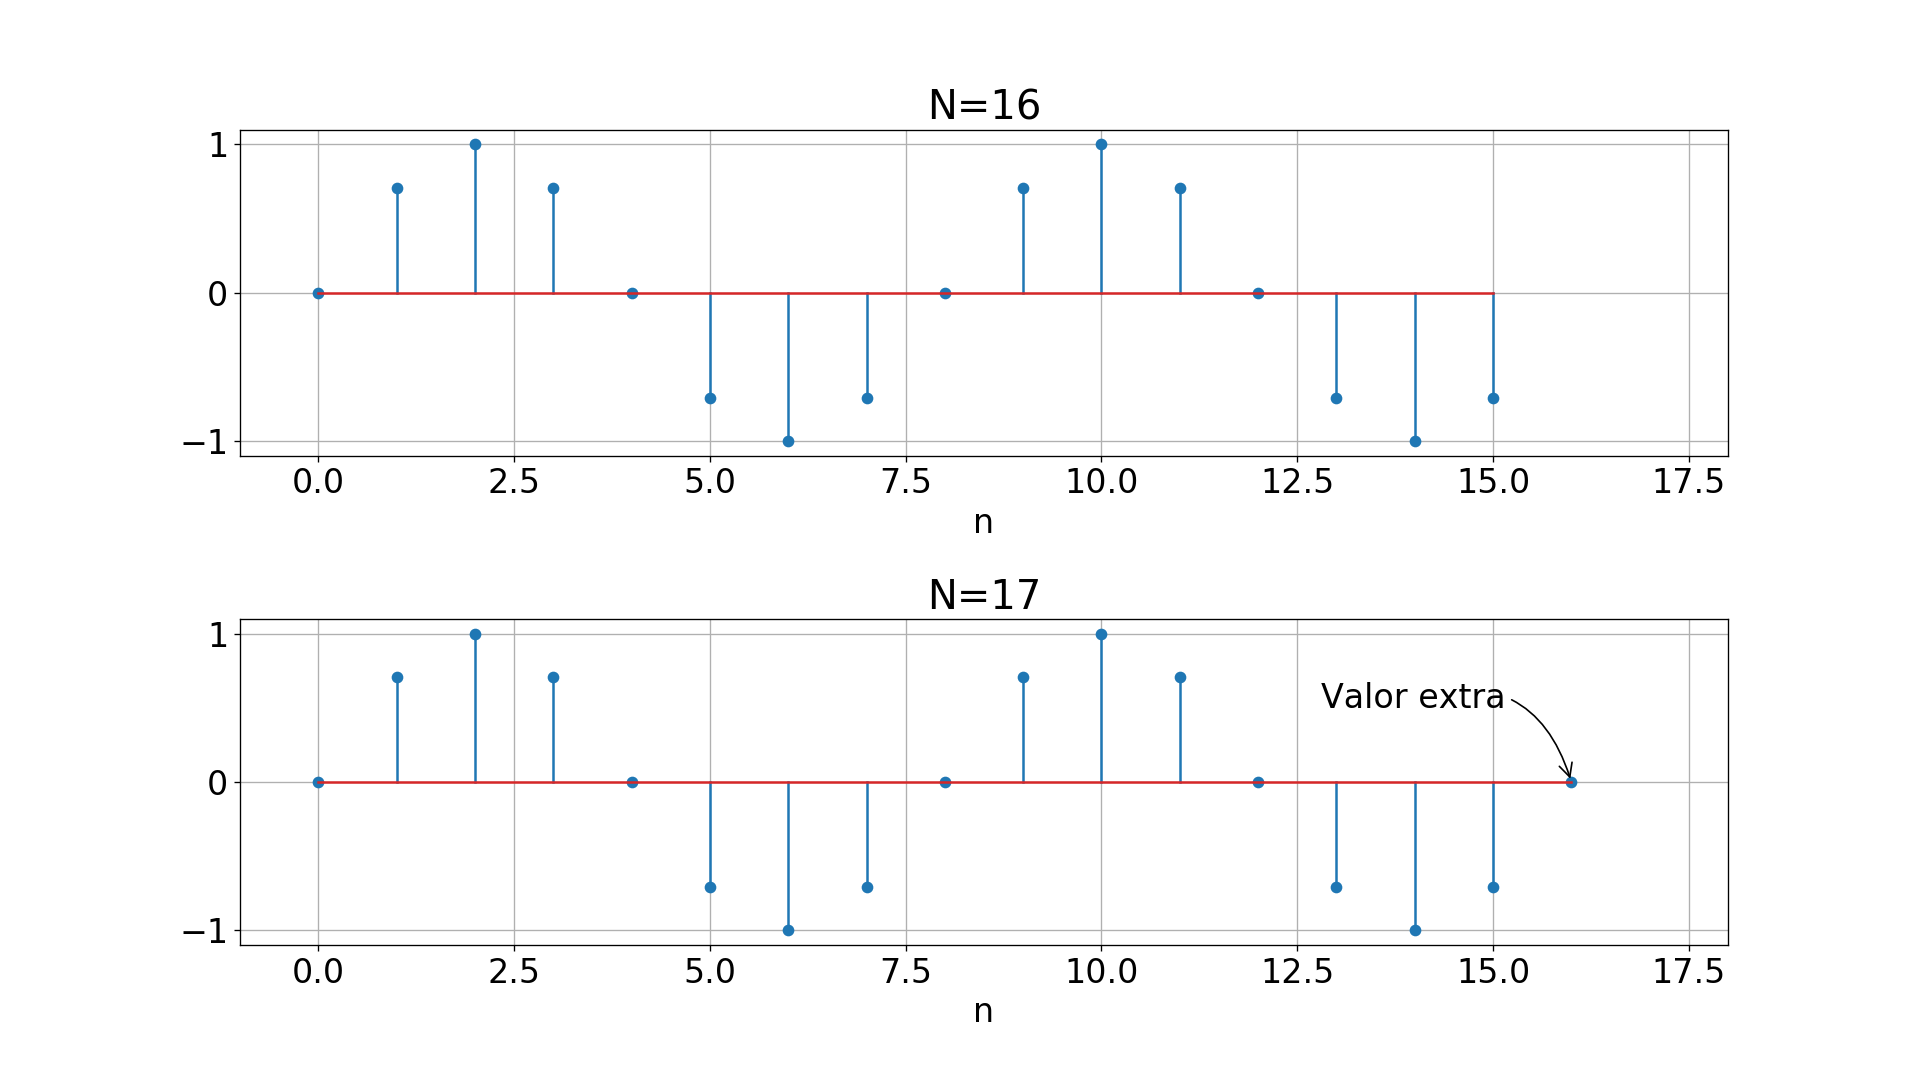
\includegraphics[width=0.75\textwidth]{Img/punto_1_dato_de_mas.png}
\caption{DFT de la señal $x[n]$ utilizando la \textit{fft} con N=16 y N=17.}
\label{fig.2e}
\end{figure}

Analizando la Figura \ref{fig.1e} es importante destacar que el espectro generado con un valor de N=161 se aproxima mejor al espectro original que el generado con un valor de N=17. Esto sucede ya que para N=161, en la señal reconstruida por la \textit{fft} hay un solo valor erróneo cada 161 valores, con respecto a la señal original. Asimismo, si N=17 hay un error cada 17 muestras, y por lo tanto, el error acumulado es mucho mayor.


\subsection*{Inciso f)}
A raíz de las conclusiones que se obtuvieron en los incisos anteriores, las condiciones para calcular la DTFS de una señal periódica y discreta usando la \textit{fft} son las siguientes:
\begin{itemize}
    \item El valor de $N$, el cual representa la cantidad de muestras consecutivas que se otorgan como información para el cálculo de la DFT, mediante \textit{fft}, debe ser un múltiplo del periodo fundamental de la señal. Caso contrario, el algoritmo construirá una señal diferente, al replicar un período erróneo.
    \item El resultado que entrega la función \textit{fft} no está escalado por el factor $\frac{1}{N}$. Por consiguiente, se debe tener en cuenta este escalado de amplitud al momento de querer obtener los $c_{k}$ de una señal periódica y discreta a partir de la \textit{fft}.
\end{itemize}

\subsection*{Inciso g)}
Para el uso correcto de la función \textit{fftshift} se debe generar un vector que contenga las muestras de la señal centradas en cero: $n_{centrado}=-N/2:1:N/2$, donde $N$ es la cantidad de muestras de la señal discreta. Posteriormente, utilizar el vector generado de forma centrada al momento de implementar el gráfico con la función \textit{plot}. Cabe destacar que si $N$ es impar, se debe utilizar el comando \textit{Round} para redondear el resultado de los límites en el vector $n_{centrado}$.

En la Figura \ref{fig.1g} y \ref{fig.2g} se pueden visualizar los resultados obtenidos en los incisos \textbf{b)} y \textbf{c)} respectivamente, utilizando esta vez, la función \textit{fftshift}.

\begin{figure}[H]
\centering
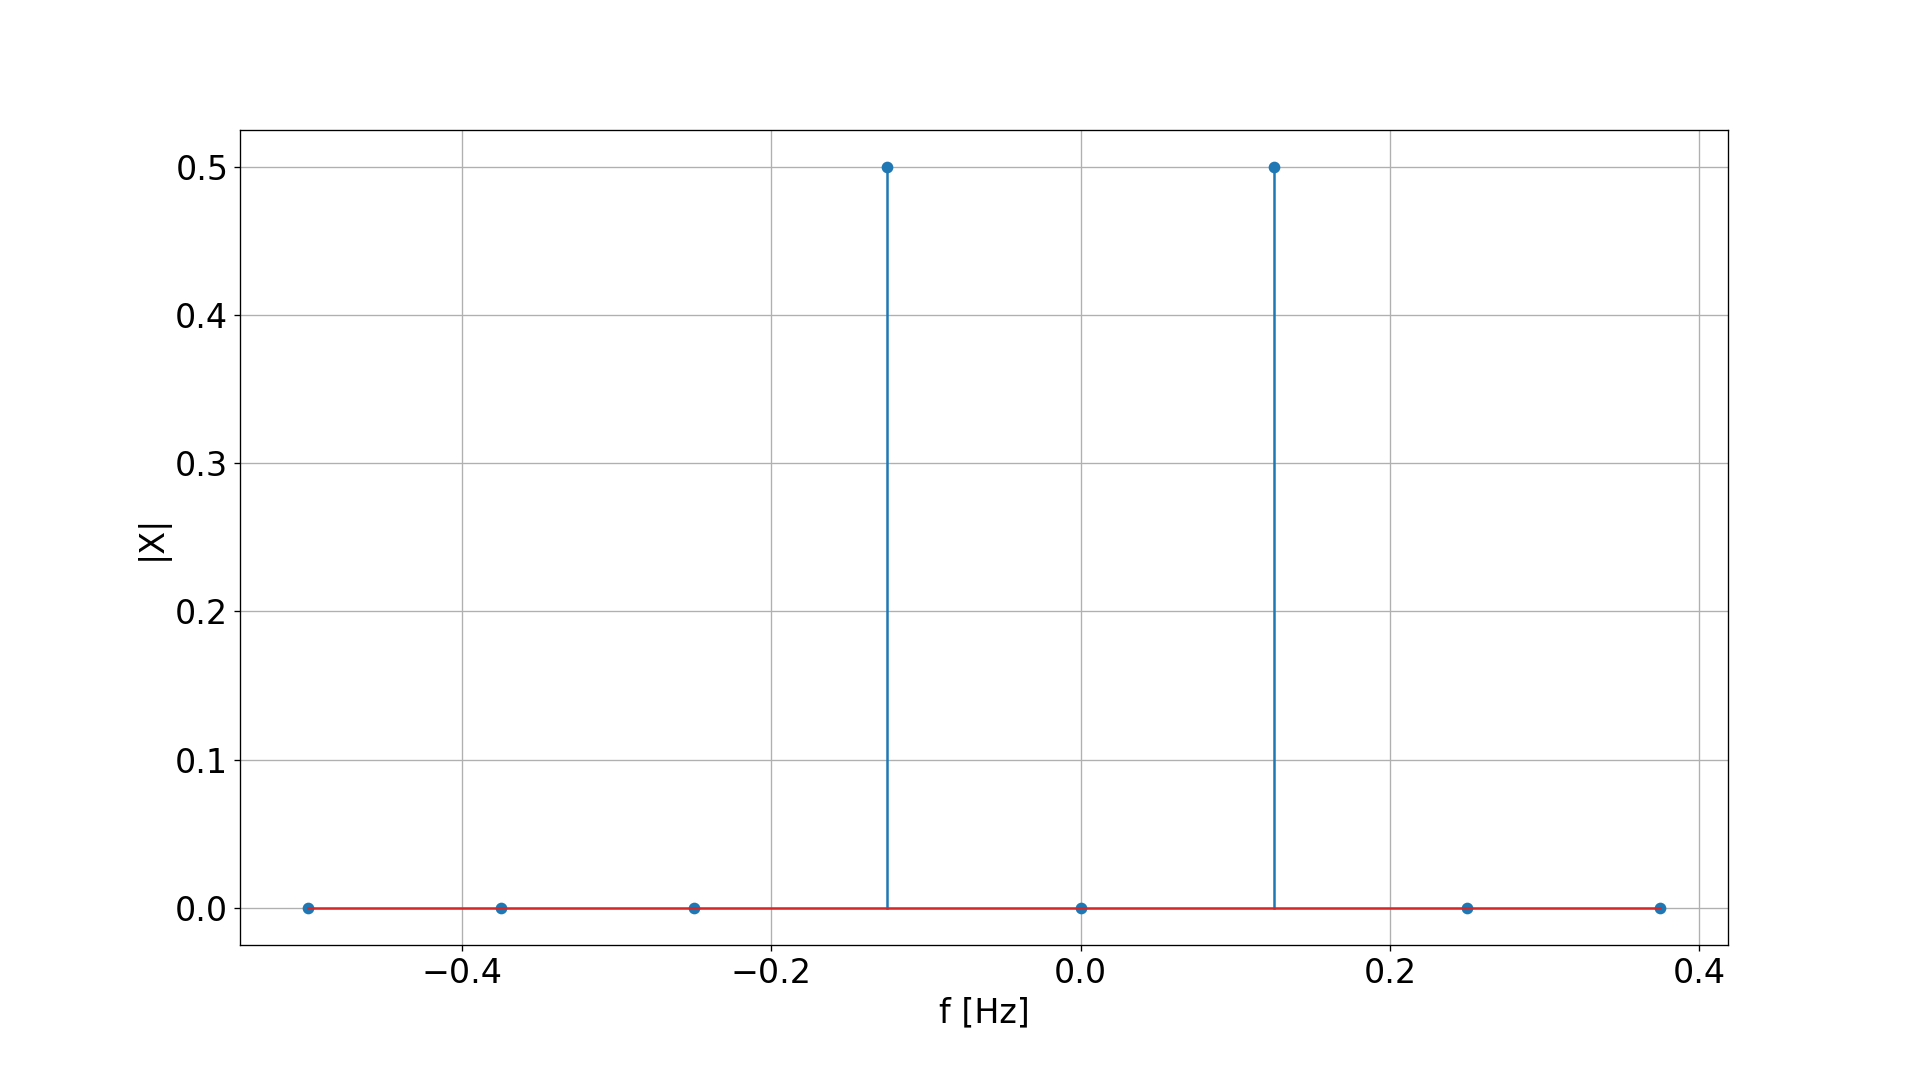
\includegraphics[width=0.75\textwidth]{Img/punto_1_g_a.png}
\caption{DFT de la señal $x[n]=sen(2 \pi n /8)$ con N de 0 a 7, centrada con la función \textit{fftshift}.}
\label{fig.1g}
\end{figure}

\begin{figure}[H]
\centering
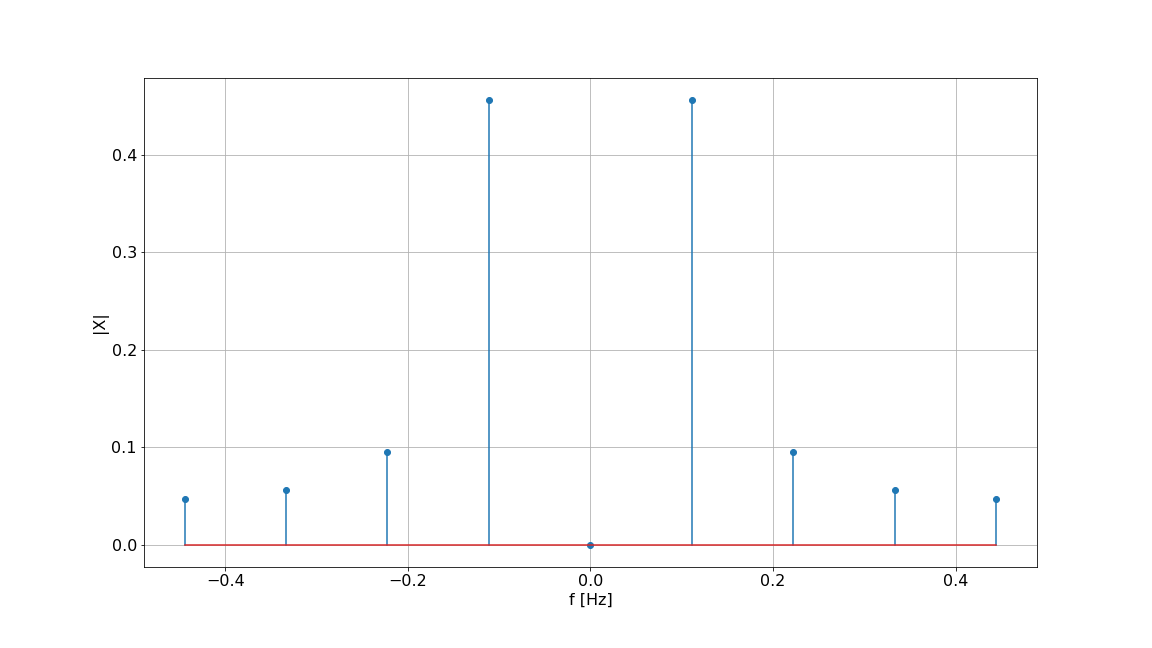
\includegraphics[width=0.75\textwidth]{Img/punto_1_g_b.png}
\caption{DFT de la señal $x[n]=sen(2 \pi n /8)$ con N de 0 a 8, centrada con la función \textit{fftshift}.}
\label{fig.2g}
\end{figure}



\subsection*{Inciso h)}



\subsubsection*{i)}

\begin{equation}
    x_1[n]= sin(2\pi n/7) + 2cos(4 \pi n /7) + 3sin(6\pi n/7)
\end{equation}


Utilizando la identidad de \textit{Euler}:
\begin{equation}
    x_1[n]= \frac{e^{j2\pi n/7} - e^{-j2\pi n/7} }{2j} +  e^{j4\pi n/7} + e^{-j4\pi n/7} + \frac{3e^{j6\pi n/7} - 3e^{-j6\pi n/7} }{2j}
\end{equation}

Por lo tanto los coeficientes son:
\begin{table}[H]
    \centering
    \begin{tabular}{|c|c|c|c|c|c|c|c|}
        \hline
        $k$ & -3 & -2 & -1 & 0 & 1 & 2 & 3  \\ \hline
        $c_k$ & $-j3/2$ & $1$ & $-2j$ & 0 & $2j$ & $1$ & $j3/2$ \\ \hline
        \end{tabular}
    \caption{Coeficientes $c_k$.}
    \label{}
\end{table}

\subsubsection*{ii)}
\begin{equation} 
    x_{2}[n] = \left\{ 
    \begin{array}{ll} 
    1 & \mathrm{si\ } 10 k - 2\\
    0 & \mathrm{sino\ } \\
    \end{array} 
    \right.
\end{equation}
 
Del conocimiento previo de señales y sistemas se sabe que los coeficientes de la serie son valores muestreados de un sinc.

\subsubsection*{iii)}

\begin{equation} 
    x_{3}[n]=\sum_{l=-\infty}^{\infty}\delta{n-3-20 l} 
\end{equation}
\begin{equation} 
    c_{k}=\frac{1}{N} \sum_{n=0}^{N-1}\sum_{l=-\infty}^{\infty} \delta{n-3-20 l}  e^{\frac{-2 \pi n k j }{N}}
\end{equation}

La segunda sumatoria desaparece ya que se analiza solo un periodo de la señal, por conveniencia se toma k=0.

\begin{equation} 
    c_{k}=\frac{1}{N} \sum_{n=0}^{N-1}\delta{n-3}  e^{\frac{-2 \pi n k j }{N}}
\end{equation}
\begin{equation} 
    c_{k}=\frac{1}{N}  e^{\frac{-6 \pi  k j }{N}}
\end{equation}
\begin{equation} 
    c_{k}=\frac{1}{20}  e^{\frac{-3 \pi  k j }{10}}
\end{equation}
Donde la exponencial que multiplica al término $\frac{1}{20}$ implica un desplazamiento en la frecuencia de los coeficientes.


%ARRANCA EL PUNTO 2

\section{Ejercicio 2}

    En este ejercicio se analiza el caso de que una señal es periódica y continua. Para realizar el análisis se utiliza la siguiente señal: 

    \begin{equation}
        \label{eq.punto2}
        x_c(t) = sin( 200 \pi t )
    \end{equation}

    \subsection*{Inciso a)}

    En este inciso se calcula la CTFS de eq.\ref{eq.punto2}. Se sabe con anterioridad que la CTFS de una señal
    esta definida:
    
    \begin{equation}
        x(t)= \sum_{k=-\infty}^{\infty} a_k e^{j\omega_0 kt}
    \end{equation}

    \begin{equation}
        a_k = \frac{1}{T} \int_{-T/2}^{T/2} x(t)e^{-j\omega_0 kt}
    \end{equation}

    Aplicando la fórmula de Euler a la eq.\ref{eq.punto2} se obtiene:

    \begin{equation}
        x_c(t)=\frac{1}{2j}( e^{j200\pi t} - e^{-j200 \pi t})
    \end{equation}

    Es posible apreciar que los coeficientes de la serie son: 

    \begin{equation}
        c_1 = \frac{1}{2j} \hspace*{.1cm} \land \hspace*{.1cm} c_{-1}=-\frac{1}{2j}
    \end{equation}

    \subsection*{Inciso b)}

    En este inciso se muestrea la señal a una frecuencia adecuada, y luego se le calcula de DFT.

    Aplicando el teorema del muestreo, se debe elegir una frecuencia mayor a $2F_N$, siendo 
    en este caso $F_N=100Hz$, por ello se utilizara $F_s=400Hz$. Con dicha frecuencia se obtiene 

    \begin{equation}
        x[n]=x(n/F_s) \rightarrow x[n]= sin\left( \frac{\pi}{2} n\right)
    \end{equation}

    Cuyo período fundamental ($N_0$) es $4$.

    Aplicando la ecuación (\ref{eq.DFT}):

    \begin{equation}
        X[k]= \sum_{n=0}^{3} sin\left( \frac{\pi}{2} n\right) e^{-j\frac{\pi}{2} nk}
    \end{equation}

    Calculando los valores de $x[n]$ para $n\in {1, 2, 3 ,4}$

    \begin{table}[H]
        \centering
            \begin{tabular}{|c|c|c|c|c|}
            \hline
            $n$ & 0 & 1 & 2 & 3  \\ \hline
            $sin(\pi n/2)$ & 0 & 1 & 0 & -1 \\ \hline
            \end{tabular}
        \caption{Valores de la señal muestreada en un periodo.}
    \end{table}

    Reemplazando en la ecuación anterior, se obtiene:

    \begin{equation}
        X[k]= e^{-j\frac{\pi}{2}k} - e^{-j\frac{ 3 \pi}{2}k}
    \end{equation}

    Es posible expresar a $e^{-j\frac{ 3 \pi}{2}k}$ como $e^{-j \frac{\pi }{2}k}e^{-j\pi k}$, aplicando la identidad de Euler 
    $e^{-j \pi k}= (-1)^k$. 

    \begin{equation}
        X[k]= [ 1 + (-1)^{k+1} ] e^{ -j \frac{\pi }{2} k }
    \end{equation}

    \begin{table}[H]
        \centering
        \begin{tabular}{|c|c|c|c|c|}
            \hline
            $k$ & 0 & 1 & 2 & 3  \\ \hline
            $X[k]$ & 0 & $-2j$ & 0 & $2j$ \\ \hline
            \end{tabular}
        \caption{Valores de $X[k]$.}
        \label{tab.xk}
    \end{table}

    \subsection*{Inciso c)}

    En este inciso se analiza la relación entre la CTFS y DFT, y si es posible calcular la CTFS a partir de la CTFS sin error.

    Al dividir los coeficientes $X[k]$ (Tab.\ref{tab.xk}) por el el número de muestras $N$, el resultado son los coeficientes 
    $c_k$. Luego se puede establecer a priori la relación:
    
    \begin{equation}
        c_k = \frac{X[k]}{N}
    \end{equation}

    Para la ecuación anterior se aplica el conocimiento que $X[k]$ es periódica, y por lo tanto $X[-1]=X[3]$.

    Cabe mencionar que si la señal se encuentra correctamente muestreada (cumple el teorema de muestreo) y en el caso de que la señal sea de banda limitada (tenga un número finito de 
    armónicos) como en este caso, se puede obtener de manera exacta la aproximación sin error. Pero en el caso de tener una señal que no sea de banda limitada (como el caso de un cajón) se tendria un error debido 
    a que no es posible cumputacionalmente realizar el cálculo con infinitos valores.


    \subsection*{Inciso d)}

    En este inciso se genera una cantidad entera de períodos de la señal muestreada,
    para luego calcular la DFT y verificar las conclusiones obtenidas en el inciso anterior.

    \begin{figure}[H]
        \centering
        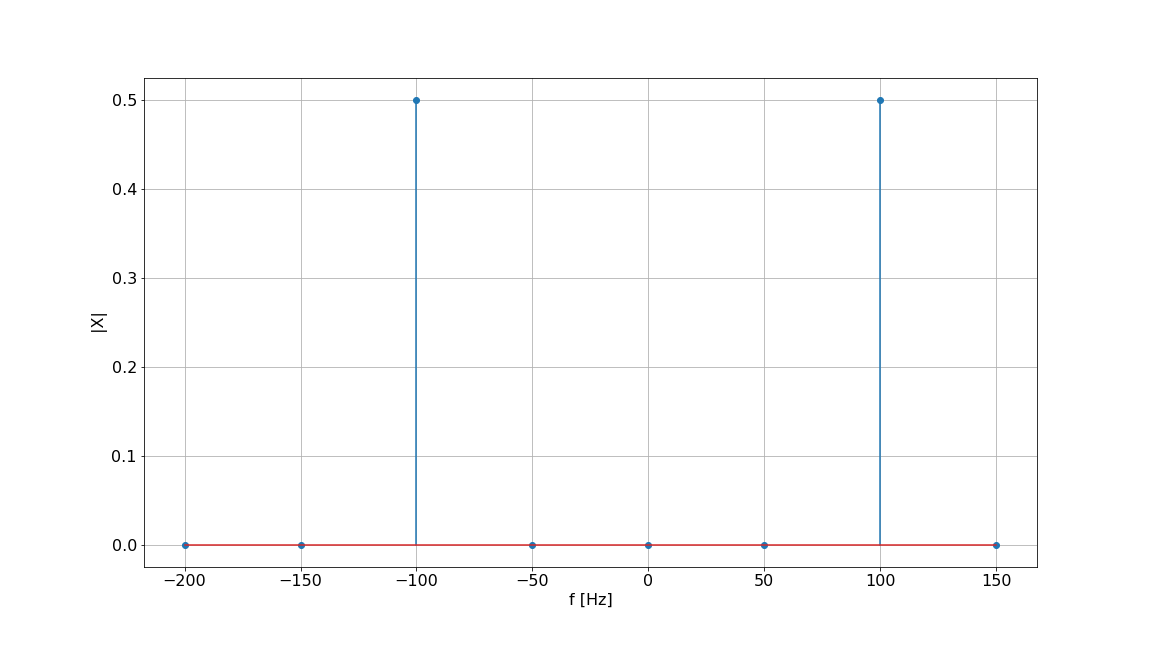
\includegraphics[width=0.75\textwidth]{Img/punto_2_d.png}
        \caption{CTFS obtenida mediante el algoritmo de FFT para N=4.}
        \label{fig.2d}
    \end{figure}
    Es posible obervar en la Fig.\ref{fig.2d} se cumple la ide previa concebida em el inciso anterior.
    
    \subsection*{Inciso e)}

    En este inciso se agrega una muestras más, y se analiza lo que sucede con la DFT.

    \begin{figure}[H]
        \centering
        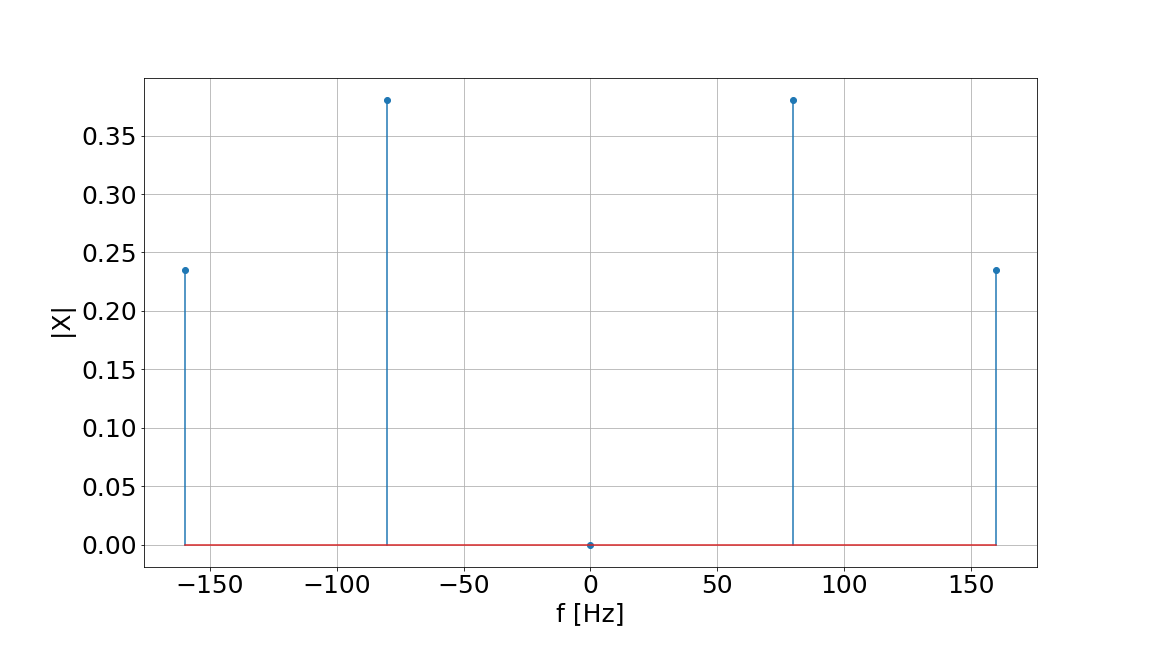
\includegraphics[width=0.75\textwidth]{Img/punto_2_e.png}
        \caption{CTFS obtenida para N=5}
        \label{fig.2e}
    \end{figure}

    Al añadir una muestra mas a la señal ingresada, debido a como se implementa el algoritmo, la señal se ve modificada y su 
    extensión periódica es diferente, similar a lo que sucedió en el inciso 1-e, por lo que se observa en la Figura \ref{fig.2e} aparecen valores de frecuencia que no son los esperados; este error debido a como se implementa la DFT, ya que el algoritmo ve una señál de periodo 5, en este caso, la cual no representa la señal real, y por lo tanto el espectro no coincide con el de la señal original.


    \subsection*{Inciso f)}

    En este inciso se establecen las condiciones para poder obtener de forma exacta la 
    CTFS a partir de la DFT.

    Para obtener la CTFS usando la FFT, es necesario realizar un buen muestreio de la señal, 
    para obtener la señal muestrada. A dicha señal se apalica la FFT con el número correspondiente
    de puntos (se debe cumplir que el número de puntos tomados sea mayor o igual al número mínimo de puntos que representa un periodo de la señal). 
    Posteriormente se normaliza con el valor de puntos 
    y de esa manera se obtiene la CTFS aproximada aplicando la FFT.

    Por otro lado, para que la representación sea exacta se deben cumplir las siguientes condiciones:
    \begin{enumerate}
        \item La señal original debe ser de banda limitada.
        \item Se debe muestrear respetando el teorema de muestreo $F_s\geq 2F_N$
        \item El número de puntos que se usan en la FFT debe ser un múltiplo del número de muestras que representan un período ($N\geq L$)
    \end{enumerate}

    \subsection*{Inciso g)}

    En este inciso se comprueba de forma práctica las conclusiones obtenidas en 
    el inciso anterior, las siguientes señales 
    
    \begin{enumerate}
        \item $x_1(t)= 4 sen( 2\pi 1000 t ) + 3sen( 2\pi 2000 t ) + 2sen( 2\pi 3000 t )$
        \item $ x_2(t)= \sum_{l=-\infty}^{\infty} \mu( t - 10l - 2  )\mu( 2 + 10l - t )$
    \end{enumerate}

    \subsubsection*{i)}

    Para poder comparar y verificar el correcto funcionamiento del algoritmo de FFT
    se buscara la CTFS de forma teorica, para ello se aplica la formula de Euler
    
    \begin{equation}
        x_1(t) = \frac{1}{2j} ( 4e^{j2000 \pi t} - 4e^{-j2000 \pi t}  +3e^{j4000 \pi t} - 3e^{-j4000 \pi t} +2e^{j6000 \pi t} - 2e^{-j6000 \pi t} )
    \end{equation}

    

    Por lo que se obtienen los coeficientes de la serie de forma sencilla de la Tabla (\ref{tab.2gi}).

    \begin{table}[H]
        \centering
        \begin{tabular}{|c|c|c|c|c|c|c|c|}
            \hline
            $k$ & -3 & -2 & -1 & 0 & 1 & 2 & 3  \\ \hline
            $c_k$ & $j$ & $3j/2$ & $2j$ & 0 & $-2j$ & $-3j/2$ & $-j$ \\ \hline
            \end{tabular}
        \caption{Coeficientes $c_k$.}
        \label{tab.2gi}
    \end{table}

    Para calcular la DFT se debe seleccionar una frecuencia de muestreo, debido a que la frecuencia máxima de la señal es de $3000Hz$ se toma $F_s = 9000 muestras / seg$.

    \begin{figure}[H]
        \centering
        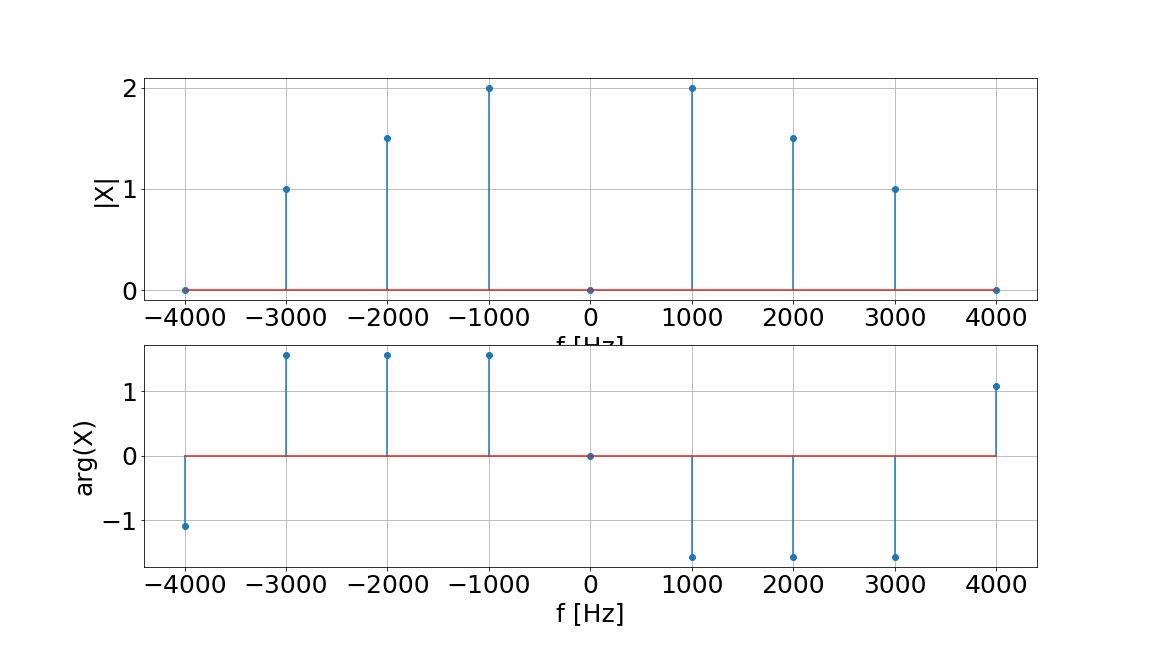
\includegraphics[width=0.75\textwidth]{Img/punto_2_g_1.png}
        \caption{CTFS de $x_1(t)$ obtenida con el algoritmo de FFT.}
        \label{fig.2gi}
    \end{figure}
    
    \subsubsection*{ii)}

    Dicha ecuación describe un tren de pulsos de ancho $4$ y periodo $10$, al calcular los coeficientes de la CTFS se obtienen
    infinitos valores cuya envolvente es una $sinc$, debido a que la señal no es de banda limitada no sera posible recuperara su espectro 
    de forma completa. 

    \begin{equation}
        a_k = \frac{4}{10} sinc \left( \frac{2}{4}k \right)
    \end{equation}

    Debido a que no es posible recuperar el espectro de la señal original, pero si aproximarlo, se toma $F_s=5 muestras/seg$, para
    obtener una aproximación aceptable, en caso el período de la señal muestreada sera de $50 muestras$.

    \begin{figure}[H]
        \centering
        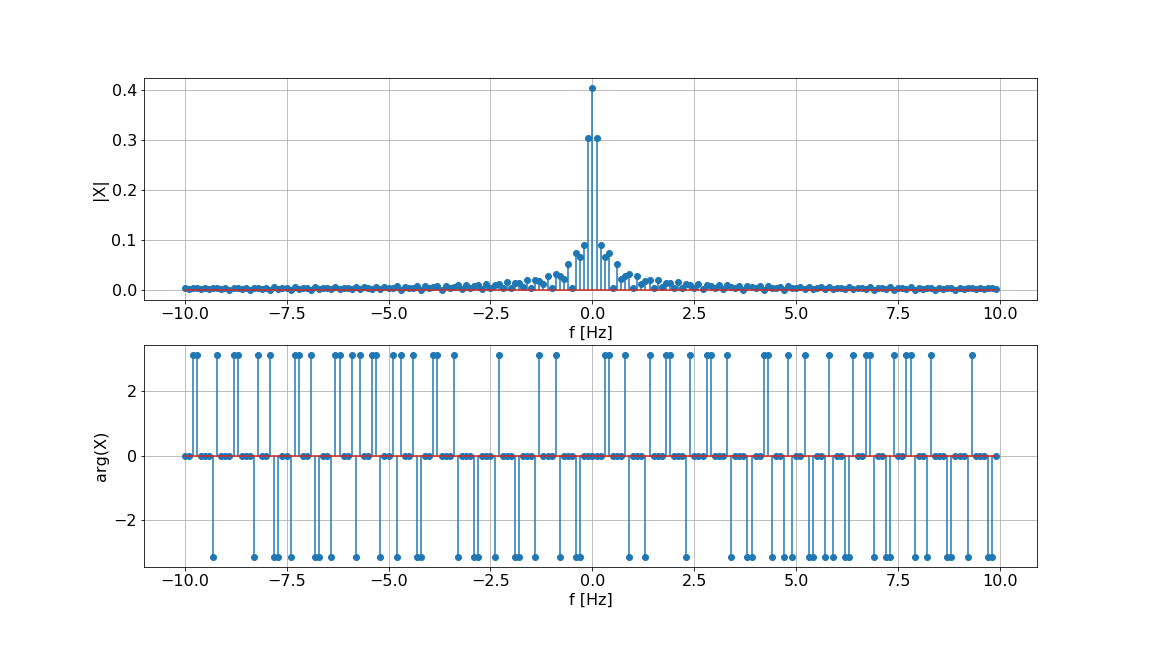
\includegraphics[width=0.75\textwidth]{Img/punto_2_g_2.png}
        \caption{CTFS de $x_2(t)$ con $F_2=5 muestras/s$ y $N=50$ y la envolvente.}
        \label{fig.2gii}
    \end{figure}

    En la Figura \ref{fig.2gii} se observa como los valores de los coeficientes obtenidos difieren con los valores reales. No obstante, se puede concluir que dicha aproximación es útil para estimar el espectro. De forma adicional se incluye un \href{https://drive.google.com/open?id=10pVC59n6z_zfX6Qlm4w96l_1q3lnr2g6}{\underline{video}}
    donde es posible observar como al variar $F_s$ los coeficientes de la CTFS se ajustan cada vez mejor a los valores de la envolvente. Cabe destacar que nunca se podrá obtener de forma exacta la CTFS, pero si es posible lograr una muy buena aproximación. 

\end{document}